\documentclass{report}
\usepackage[utf8]{inputenc}
\usepackage[margin=1in]{geometry}

\usepackage{amssymb}
\usepackage{listings}
\usepackage{algorithm}
\usepackage{algorithmic}
\usepackage{color}
\usepackage{graphicx} %package to manage images

%New colors defined below
\definecolor{codegreen}{rgb}{0,0.6,0}
\definecolor{codegray}{rgb}{0.5,0.5,0.5}
\definecolor{codepurple}{rgb}{0.58,0,0.82}
\definecolor{backcolour}{rgb}{0.95,0.95,0.92}

%Code listing style named "mystyle"
\lstdefinestyle{mystyle}{
  backgroundcolor=\color{backcolour},   commentstyle=\color{codegreen},
  keywordstyle=\color{magenta},
  numberstyle=\tiny\color{codegray},
  stringstyle=\color{codepurple},
  basicstyle=\footnotesize,
  breakatwhitespace=false,         
  breaklines=false,                 
  captionpos=b,                    
  keepspaces=true,                 
  numbers=left,                    
  numbersep=5pt,                  
  showspaces=false,                
  showstringspaces=false,
  showtabs=false,                  
  tabsize=2
}

%"mystyle" code listing set
\lstset{style=mystyle}

\begin{document}

\title{EECE 7360 Project 5 \\
  Subset Sum}
\author{Garrett Goode and Daniel Hullihen}
\maketitle

%%%%%%%%%%%%%%%%%%%%%%%%%%%%%%%%%%%%%%%%%%%%%%%%%
% INTRODUCTION
%%%%%%%%%%%%%%%%%%%%%%%%%%%%%%%%%%%%%%%%%%%%%%%%%

\chapter{Introduction}
The subset sum problem (also referred to as the ``exact knapsack problem'')
is defined below.

\textit{Let A = $\{a_1, ..., a_n\}$ represent some set of integers. Given a sum s, find a subset $A' \subset A$ such that
  $$s = \sum_{i=1}^m a'_i, for 1 \le i \le m.$$
  Where m is the size of $A'$.}
  
In other words, if we are given a list of numbers and some target sum, we want
to find the numbers in the list that add up to the target sum. Put as a decision
problem, the question would be ``Is there a subset A' of A where the sum of the
elements of A' is s?''

In this project, several approaches for solving instances of the subset
sum problem were investigated and compared against each other.
Benchmarks were developed based on prior work,
and background research was done to highlight subproblems of subset sum.
Exhaustive and greedy solvers were implemented and evaluated. Linear
programming (LP) and integer-linear programming (ILP) models were developed
and evaluated as well. Lastly, local search algorithms were implemented,
evaluated and compared to all other previous implementations.

%%%%%%%%%%%%%%%%%%%%%%%%%%%%%%%%%%%%%%%%%%%%%%%%%
% PROJECT 1
%%%%%%%%%%%%%%%%%%%%%%%%%%%%%%%%%%%%%%%%%%%%%%%%%
\chapter{Benchmarking}
Before any benchmark or instances can be generated, it is necessary to understand
the prior work done to evaluate implementations of algorithms that solve the
subset sum problem. The most popular metric used for determining the difficulty of
an instance of the subset sum problem is the ``density'' of the set in question.
The following equation
describes the density of a set.
$$d = n / log_2 max(a_i)$$
where n is the size of the set in quation and $max(a_i)$ is the largest element in the set.

Previous work has focused on being able to solve a
group of instances that had a some density \cite {lagarias1985}.
For example, Radziszowski and Kreher explored efficiently solving low density subset
sum problems ($d < 0.7$) \cite {kreher1988}. Schnorr and Euchner pointed out
``the hardest subset sum problems turn out to be those that
have a density that is slightly larger than 1, i.e. a density about
$1 + log_2(n/2))/n$'' \cite {schnorr94}.
On top of that, LaMacchia points out that subset sum problems with a density
$d < 0.6463...$ could be solved in polynomial time by a
``lattice oracle'' \cite {lamacchia91}, showing that there are existing algorithms
designed to work efficiently in certain areas of the instance space (in this
case, with a sufficiently low density). 

What this boils down to is: much research has focused on subset sum problems with
densities of and around 1.0. More recently, when evaluating a GPU
implementation of the subset-sum problem, Wan et al. crossed vector sizes of
36 to 54 containing random values in the range $[1, 10^8]$, covering a large
range of possible densities \cite {wan2015}. Thus, in order to provide a fair
comparison with prior work, we need to create instances with densities
on and around 1.0. For breadth, we should focus on sufficiently small and large
densities as well, and cover different combinations of set length and maximum
value that may yield the same density in order to see if those values
may have a disproprtionate impact on performance. 

\subsection{Instance Generation}
Given the prior work, when it comes to generating benchmarks for evaluating different
implementations of the subset sum problem, it is necessary to focus on the density of
the instances generated, and the range of densities covered by the overall suite.
152 instances were generated, with an emphasis on instances with densities around
1.0 in order to have a finer granularity of data. To generate each instance, we
determined the number of elements needed in the set, as well as the largest
value that will exist in the set (determined by the number of bits it represents).
For each generated number in the set, b bits of random value 0 or 1 were generated.
These bits were then concatenated together to form an interger.
Once the list was complete, we randomly chose exactly half of the elements in the
list and added them up. This sum is the solution for the instance.

The following table shows the different groups of instances that were generated
and some properties that were derived from them. In each row, a range of n and
b values were generated. These lists of values were crossed to generate
a group.
\begin{center}
  \begin{tabular}{| c | c | c | c | c | c |}
    \hline
    n (Start:End:Stride) & b (Start:End:Stride) & Count & Min d & Max d & Avg. d \\
    \hline
    2:10:2 & 20:26:2 & 20 & 0.076 & 0.5 & 0.263 \\
    \hline
    16:30:2 & 15:30:2 & 64 & 0.55 & 2.0 & 1.09 \\    
    \hline
    2:10:2 & 2:10:2 & 25 & 0.2 & 5.0 & 1.37 \\
    \hline
    50:100:10 & 15:30:5 & 24 & 1.66 & 6.66 & 3.5 \\    
    \hline
    90:100:2 & 2:10:3 & 18 & 11.25 & 50 & 26.125 \\    
    \hline
  \end{tabular}
\end{center}
Note it is possible to achieve the same density with different values of n and b.
In general, we aimed to cover a cross of large and small n with large and small b
(e.g. large set with small numbers, small set with large numbers, etc.). Together,
the above groups in the table span densities from as low as 0.076 to as high as 50,
covering a wider range than what was described in the literature. Given the emphasis
on cases around a density of 1.0, we argue this is representative of the instance
space and in line with prior work.

\chapter{Exhaustive Algorithm}
For the first attempt at solving the Subset Sum problem instances we had generated, we
chose an exhaustive "brute force" approach. Rather than attempt to target specific
subsets of our input set, we cycled iteratively through every possible solution.

\begin{algorithm}
  \caption{Exhaustive Algorithm to Solve Subset Sum}
  \label{exhaustive}
  \begin{algorithmic}
    \FOR{subset s in set S}
    \STATE{$sum \gets 0$}
    \FOR{element i in s}
    \STATE{$sum += element$}
    \ENDFOR
    \IF{$sum == targetSum || timeOutReached$}
    \STATE{$break$}
    \ENDIF
    \ENDFOR
  \end{algorithmic}
\end{algorithm}

Since an element in the input set can be "in" or
"out" of the solution set, there are $2^{n}$ possible subsets. Therefore, the possible
subsets can all be represented by an n-digit binary number. In our implementation of a 
data representation of a subset sum instance, we represented a solution as an array with
the same number of elements as the input set, with each entry set to "INCLUDED" or
"EXCLUDED". This representation allowed us to emulate adding 1 to a binary number,
starting with every entry set to EXCLUDED and ending when every entry was set to INCLUDED.

Given the above, it is easy to characterize the run time of our exhaustive algorithm.
There is an initiation step, and the $2^{n}$ possible solutions are looped through in the worst case. 
Additionally, generating the current sum of the solution set also requires cycling through all n of its elements. 
This yields the expression below.
$$O(n + n*(2^{n})) = O(2^{n})$$
As expected, the worst cases of Subset Sum cannot be solved exhaustively in poynomial time.

\section{Results}

The results are presented in the figure below. The vertical axis represents the
input size and the horizontal axis the word length of the elements in bits.

\begin{figure}[h]
\centering
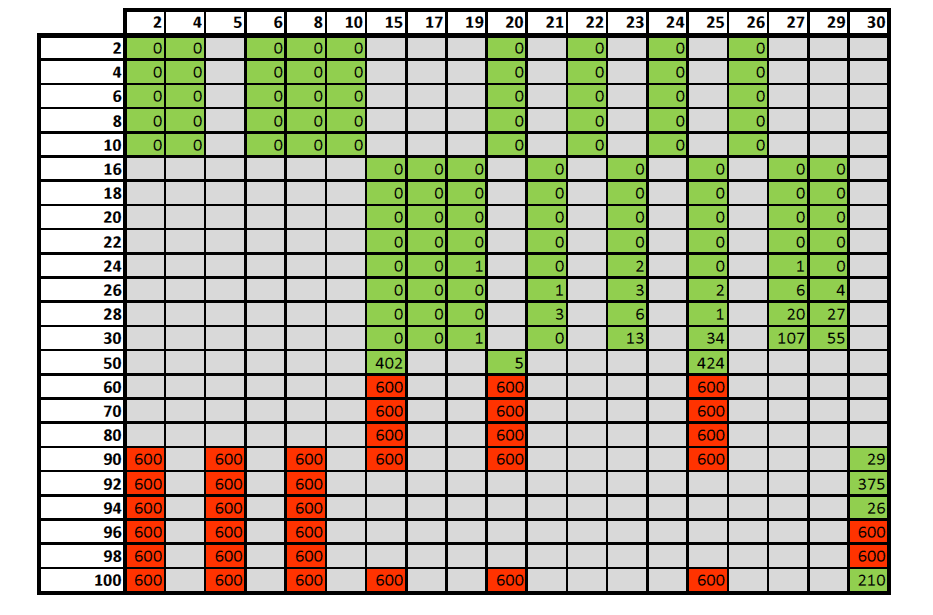
\includegraphics[width=12cm]{P1_res.png}
\caption{Run time for various input size and word length combinations}
\end{figure}

Notice that the majority of the instances were solved very quickly. And there were more
still that could be solved in less than 1 minute, namely up to an instance size of 30,
depending on the max bit-width of the elements in the set. The case with a bit-width
of 27, for example, took longer than a minute. The largest instance set that could
be solved in 1 minute or less was 94, while the largest size that could
be solved in less than 10 minutes was 100. Even then, there were instances between these
two cases that could not be solved in 10 minutes. 

As expected, the exhaustive "brute force" approach largely failed to solve
instances where $n > 50$. This is not universally true however, as the algorithm
did manage to solve a few large instances of the largest word size we tested. From 
this we can conclude that word size does not have a large impact on the run time of
the algorithm and that brute force can be viable for even some large instances.
However speaking more generally an exhaustive approach is really only viable for
smaller instances of subset sum, per both the complexity analysis in the preceeding
section and the data presented in the last figure.

\section{Conclusion}
The exhaustive algorithm is a simple algorithn to implement, but can quickly approach
its timeout. By definition every single instance will be considered
unless a timeout mechanism is used to end the solver early.
The worst-case time complexity is not realized in our experiments until the instance
size was greater than 60 elements. Even at 50 elements the algorithm began to show
signs of struggle. In general, the density of the instance did not
impact the run-time of this algorithm; instead, the algorithm was largely impacted by the
instance size.

%%%%%%%%%%%%%%%%%%%%%%%%%%%%%%%%%%%%%%%%%%%%%%%%%
% PROJECT 2
%%%%%%%%%%%%%%%%%%%%%%%%%%%%%%%%%%%%%%%%%%%%%%%%%
\chapter{Survey of Complexity Landscape}
In this chapter, we explore the complexity landscape around the subset sum
problem, including subproblems to subset sum, as well as problems of which
which subset sum is itself a subproblem. Identifying possible subproblems can be helpful
when it comes to deciding which kind of algorithm is best used to solve it, as it
could possibly exploit some unique property to that subproblem.

\section{Natural Subproblems of Subset Sum}
The subset sum problem can be solved in pseudo-polynomial time, which means
there are subproblems to subset sum that can be solved in polynomial time,
but the ``hardest'' subproblem in subset sum is nevertheless NP-Complete. Due
to this property, it is possible to detect some subproblems to subset
sum and apply a known algorithm that solves the problem in polynomial time.
Some algorithms used for solving subset sum use a divide-and-conquer
approach and identify these subproblems. Subproblems
to subset sum, for example, can have all numbers that have some special
property, or the set of numbers itself has some property that can be
exploited.
This section explores some of the natural subproblems to subset sum. 

\subsection{Sets with a low density}
One metric for describing an instance of subset sum is
the density of the set. The following equation
describes the density of a set.
$$d = n / log_2 max(a_i)$$
where n is the size of the set in quation and $max(a_i)$ is the largest
element in the set.
Lagarias and Odlyzko found that, for sets that have a density less than 0.645,
their ``Algorithm SV'' can solve the instance in polynomial
time \cite{lagarias1985}. One of the steps in their algorithm involves
taking set and perform a transformation in order to apply an
algorithm developed by Lenstra, Lenstra, and Lovasz, which has a time
complexity of $O(n^{12}+n^9(log|f|^3))$ \cite{lenstra1982}. The transformed
problem is one where a short vector e must be found within an integer lattice
L = L(a,M)

\subsection{Sets where all the numbers are coprime to m}
This approach (as well as the prior approach) focus on sets that are finite
cyclic groups, defined as $\mathbb{Z}_m = {0, 1, ..., m-1}$ of order m.
Koiliaris and Xu argue that, given a set $S \subseteq U(\mathbb{Z})_m$, which
describes a set of integers that are coprime to some integer m, finding
the set of all subset sums can be donyge with a time complexity of
$O(min(\sqrt{n}m,m^{5/4})log m log n)$ \cite{koiliaris2016}.
Note that an integer x is
coprime to m if the greatest common denomintor of the two values is 1.
As Koiliaris explains, the method behind the speed-up with this approach
is the ability to partition the set into different subsets such that ``every
such subset is contained in an arithmetic progression of the form
x, 2x, ..., lx''. With this, one can calculate the subset sums very quickly
by scaling l accordingly. These sums can then be added together. This is
only doable if m is a prime number, or if all the numbers are relative prime
to m.

\subsection{Set is a subset of $Z_m$}
Koiliaris and Xu are able to take the previous case and take it a step further,
developing an algorithm that finds all of the subsets of a set S in with a
time complexity of $O(min(\sqrt{n}m,m^{5/4})log^2m)$  \cite{koiliaris2016}.
This is for sets $S \subseteq \mathbb{Z}_m$, which is slightly different from
the previous case in that the elements of the set no longer have to be
coprime to some integer m.
Their algorithm involves recursively computing a partial subset sum
as they work across subsets of the original set.

\subsection{Set size $m \geq l^{1/\alpha}$ and elements are distinct}
Chaimovich, Freiman and Galil found that, if they took the subset sum
problem and restricted it such that $max{a_i | a \epsilon A} \leq l \leq
m^\alpha)$ (where l is some bound and m is the number of variables in the set),
then the instance could be solved with a time complexity of $O(lm^2)$
\cite{chaimovich1989}. One unique
feature of their algorithm is that supports large sets (previous algorithms
could only handle moderately large sets). The main approach in their algorithm
is, assuming $A^*$ is defined as ${S_b | B \subseteq A}$, and $S_b$ is
defined as $\sum_{a_i\epsilon B} a_i$, characterize $A^*$ as ``a small
collection of
arithmetic progressions.'' 

\section{Problems of which Subset Sum is a Natural Subproblem}

We were unable to identify any problems of which Subset sum is a natural subproblem.
However rather than ignore this area of investigation entirely, we chose to explore
similar problems that are close neighbors via transformation in the landscape of common
NP-complete problems.

\subsection{Satisfiability} 

While Satisfiability (SAT) is a few transformations away from Subset Sum on the 
complexity landscape we have presented, establishing this link between subset sum and SAT is
crucial as almost all NP completeness proofs are derived from Cook's original proof for SAT and
some transformations. The problem is defined below.

\textit{Given a set of U variables, collection of C clauses over U, is there a satisfying truth assignment for C?}

As proven by Cook in the aforementioned paper, SAT is NP-complete.

\subsection{3-Satisfiability}

Transformed from SAT, 3-Satisfiability (3SAT) is a special case of SAT where each logical 
clause can have only exactly three variables. The problem is formally defined as follows.

\textit{Given a set of U variables, collection of C clauses over U such that $|c| = 3$, is there a satisfying truth assignment for C?}

Despite this restriction on the domain of problem instances when compared to SAT, 
3SAT remains NP-complete.

\subsection{3-Dimensional Matching} 

Transformed from 3SAT, the 3-dimensional matching problem deals with finding a matching in 
a three-dimensional graph. The formal definition is given below.

\textit{Given a set $M \subset WxXxY$, where W, X, and Y are disjoint sets with the same number of elements q, does M contain a matching $M' \subset M$ such that $|M'|= q$ and no two elements are the same?}

Like the previous problems discussed in this section, 3DM remaings NP-complete in all but a few ideal scenarios.
Interestingly enough, 2-Dimensional Matching (2DM) which is not discussed at length in this seciton, is tractable.

\subsection{Partition} 

The Partition problem is defined below.

\textit{Let A = $\{a_1, ..., a_n\}$ represent some set of positive integers. Does there exist a subset $A' \subset A$ such that
  $$\sum_{a \epsilon A'} s(a) = \sum_{a \epsilon A - A'} s(a)?$$}
In other words, is there a subset of the given set with sum equal to the sum of the members of the original set not included in the subset?

Once again, the partition problem is known to be NP-Complete. Of all of the problems discussed in this section,
the partition problem is likely the closest to the Subset Sum problem. However it is not a natural subproblem of Subset Sum
as no target is given as input. Instead, the target is implied as the half of the sum of the input set.

One can see clearly how simple a transformation from an instance of Partition to and instance of Subset Sum would be however, simply
by summing the input set and setting the target total to half of the calculated sum.

\subsection{Knapsack}

The Knapsack problem is also a transformation from the Partition problem (like Subset Sum). As one might expect, the problems are
therefore very similar in nature. The Knapsack problem is defined as follows.

\textit{Given a finite set U, with each $u \epsilon U$ having an associated size s(u) and value v(u), is there a subset $U' \subset U$ such that the sum of the s(u') for all $u' \epsilon U'$ is less than a given integer K while the sum of v(u') for all  $u' \epsilon U'$ is greater than a given integer H?}

Like all of the other problems in this section, knapsack is NP-complete. There are variations of the the Knapsack problem that are
tractable, but they are not discussed in this paper as they are less related to the Subset Sum problem in question. Subset Sum itself
is sometimes refered to as the exact knapsack problem.

\section{Summary}

The chart in Figure 1 on the following page maps out all problems discussed in the preceding sections. Note that all subproblems are tractable, while all problems related by
transformation are believed to be intractable.

\begin{figure}[h]
\centering
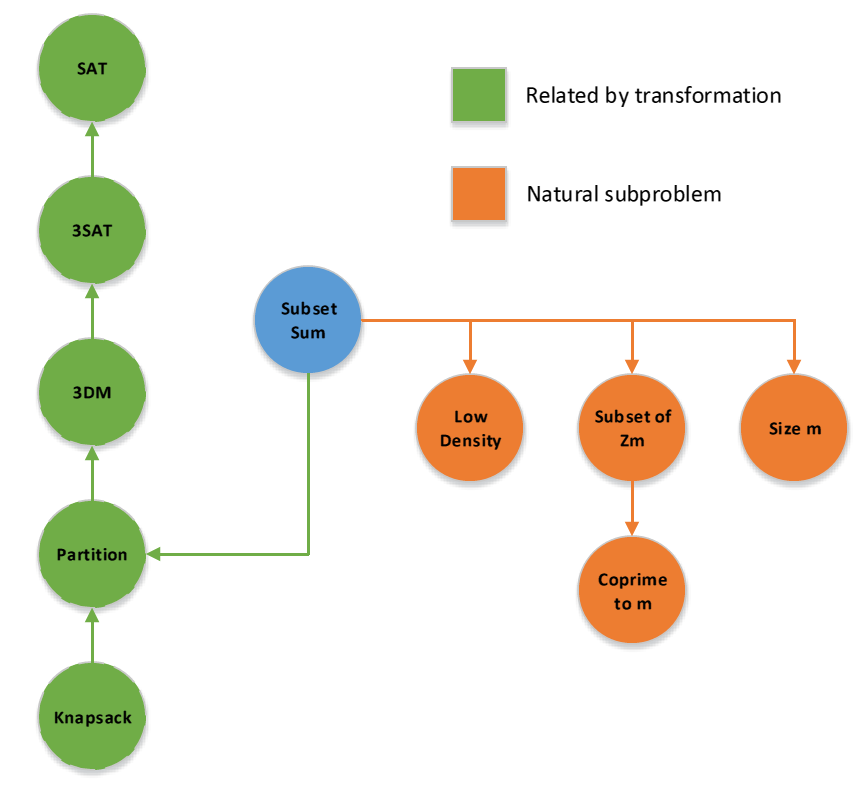
\includegraphics[width=12cm]{comp_chart.png}
\caption{Complexity landscape for Subset Sum}
\end{figure}

\section{Conclusion}

Overall the investigation into the subproblems and closely related NPC problems was very helpful in getting a clearer vision of
the nature of the Subset Sum problem. There was some some difficulty identifying problems that
subset sum was a natural subproblem of, but in the end that seemed to be apporpriate as the subset sum problem itself is very general.
It is quite simple to see how when bounds and restrictions are introduced to the origional subset sum problem statement we arrive at
various other important or interesting subproblems, but it is difficult to relax the input domain of a problem that is already so
broad and nonspecific in nature. 

%%%%%%%%%%%%%%%%%%%%%%%%%%%%%%%%%%%%%%%%%%%%%%%%
% PROJECT 3
%%%%%%%%%%%%%%%%%%%%%%%%%%%%%%%%%%%%%%%%%%%%%%%%%
\chapter{Greedy Algorithm}
In this chapter, we review an implementation of a greedy algorithm
for the subset sum problem. This implementation was run against a suite of instances, and the
performance of this algorithm is described.

\section{Greedy Algorithm Implementation}
The implementation of the greedy algorithm that was used for this project is relatively simple.
Below is the psuedocode for the algorithm.

\begin{algorithm}
  \caption{Greedy Algorithm to Solve Subset Sum}
  \label{greedy}
  \begin{algorithmic}
    \STATE{$runningSum \gets 0$}
    \STATE{$subset \gets []$} \COMMENT{Initialize subset to an empty list}
    \FOR{integer i in set S}
    \IF{$runningSum + i \le targetSum$}
    \STATE{$runningSum \gets runningSum + i$}
    \STATE{append i to subset}
    \ENDIF
    \ENDFOR
    \IF{$runningSum == targetSum$}
    \STATE{return subset}
    \ELSE
    \STATE{return NULL}
    \ENDIF
  \end{algorithmic}
\end{algorithm}

We walk through each element of the provided instance, adding numbers so long
as the running sum has not exceeded the target sum. At the end, we check to see
if the running sum matches the target sum; if it does, we have successfully solved
the instance and return the subset of integers. Otherwise we have not solved the instance
and return NULL.

One characteristic of a greedy algorithm is that, once we decide to include an element
to the sum, we never undo the decision. In the case of the subset sum problem, this
can easily cause the algorithm to not find the correct list of elements to use for the sum
since not all combinations of integers in a list are necessarily going to add up to
the target sum. Because of this, a margin of error is introduced where the algorithm
may fall short of the target sum. The upside of this algorithm is the time complexity
improvement: the algorithm visits each element of the set only once, giving the
algorithm a tightly bound time complxity of O(n). This algorithm may be useful for
applications that only need a subset that is within some percent of the target sum,
especially given the improved time complexity over the brute-force solution.

\section{Trivial Case Where the Greedy Algorithm Fails}
Due to the nature of the greedy algorithm explained in the previous section,
we can identify a trivial case where the algorithm will fail. Take for example
the set of integers S below where the target sum is 150.
$$S = \{49, 100, 50\}$$
The greedy algorithm will start from the first element and work its way through
the list, adding numbers so long as the running sum does not go beyond the target sum of 150.
In this case, the algorithm will accept the integers 49 and 100, resulting in a sum of 149.
When it encounters 50, it decides not to add this number since it would bring the running
sum over the target sum. The algorithm has then completed processing the set, but it
has failed to find a solution depite the fact one actually exists.

\section{Results}

The results are presented in Figure~\ref{fig:greedy} below. The vertical axis represents the
input size and the horizontal axis the word length of the elements in bits.

\begin{figure}[h]
\centering
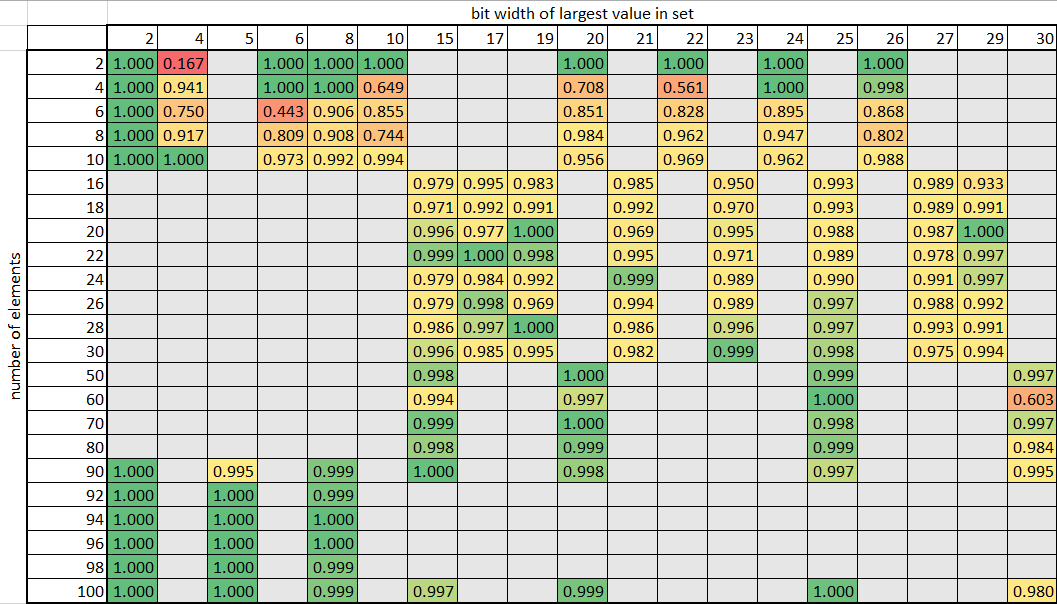
\includegraphics[width=12cm]{P3_margin.png}
\caption{Margin of error for various input size and word length combinations for the greedy algorithm}
\label{fig:greedy}
\end{figure}

Each cell in the above figure is color-coded based on the margin of error
the greedy algorithm had for the given instance. A value of 1 means the algorithm
successfully found a subset whose sum of elements matched the target sum. 
Varying yellow, orange and red elements are cases where the algorithm was more
progressively off from the target sum, with red being the most off/greatest error.

Of the 151 instances that were tested, the greedy algorithm was able to
correctly solve 28 of them, yielding an 18.5\% success rate. Compared to the
exhaustive algorithm, which had a 76\% success rate, the greedy algorithm 
is much less successful despite it's lower time complexity. As a reminder,
Figure~\ref{fig:exhaustive} shows the run-times for the exhaustive algorithm.

\begin{figure}[h]
\centering
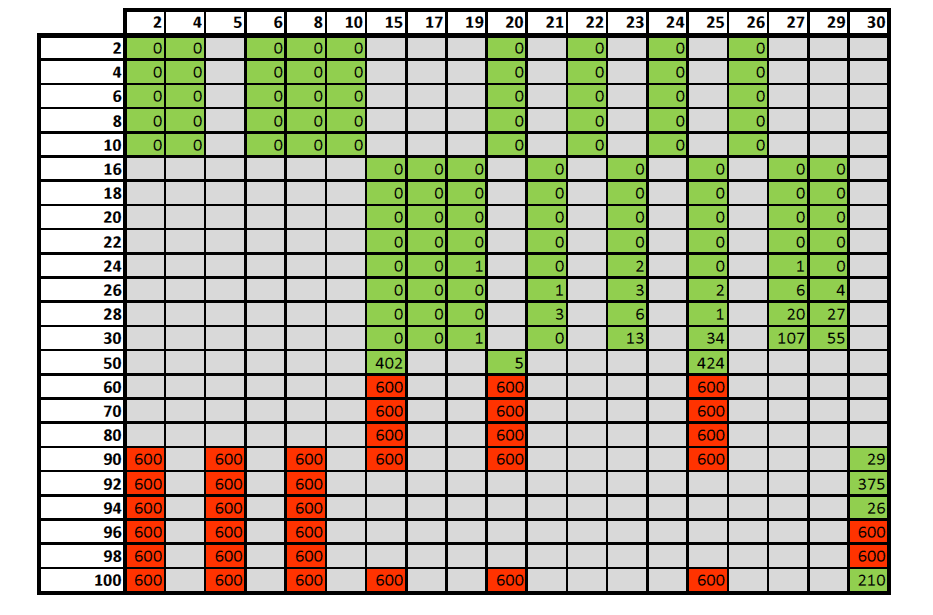
\includegraphics[width=12cm]{P1_res.png}
\caption{Run time for various input size and word length combinations for the exhaustive algorithm}
\label{fig:exhaustive}
\end{figure}

Looking at the results described in Figure~\ref{fig:greedy}, the greedy algorithm was successful
when there were sufficiently few numbers in the set, as well large sets with relatively small numbers.
For example, the majority of the instances with 90+ elements amd a max bit width < 10
passed. This may be due to the fact that, given enough sufficiently small numbers, the algorithm
can work at a small enough granularity and have a better chance to come across a total set
of numbers that can add up to the target. However, as the size of the max value increases,
the margin begins to decrease; the algorithm is less likely to hit the target sum.

The instance where the greedy algorithm had the worst margin was the one with 2 elements and a
max bit width of 4. This is most likely
due to chance. With fewer numbers, there are fewer chances to find other numbers that can add up
to the target sum. It is also a function of the distribution of numbers in the set. If there is a large
distribution of integers and the target sum actually needs the larger value, but the larger value is
at the end of the set, then the algorithm is more likely to not include it and end up with a large
margin of error. One way to possibly correct for this case is by sorting the integers from largest to
smallest before processing them.

There appears to be a sufficiently large area where the margin of error is within a few percent of the target sum,
but the algorithm nevertheless fails. This appears to happen with medium-sized sets (i.e. sets
with more than just a couple elements, but do not have a large number either). This is namely from set sizes
of about 6 to 50. The greedy algorithm is unable to correctly solve the majority of these instances.
This may be due to the fact that there are enough integers where the algorithm can accidentally add one
that will actually never allow the running sum to equal the target sum. Had there been more integers, there
would be more opportunities for the algorithm to find some other integer that could still allow
the algorithm to achieve the target sum.

In general, the amount of margin exhibited by the greedy algorithm seems to come down to how many
subsets actually do exist within the set that
satisfy the target sum, which depends on factors such as the distribution of integers values in the set
and whether a value repeats itself.
For example, for sets with several large and small numbers that are similar to each other, there may
be more subsets that satisfy a given target sum compared to a set with a more even distribution of integers.
Granted, this also depends on the target sum itself. But if there are many subsets that satisfy the
target sum, then the greedy algorithm has a better chance of solving a given instance.

\section{Conclusion}
The greedy algorithm appears to be generally effective on instances with a relatively low density. However,
it is also at the mercy of not including some element in its set that will prevent the solver from ever
being able to reach the target sum, leaving smaller instances still vulnerable to some margin of error,
regardless of the instance size itself. The margin of error decreases with suitably larger instances
since there are more opportunities to choose to include a correct element in the final set that
will bring the running total close to (if not exactly on) the target sum.

%%%%%%%%%%%%%%%%%%%%%%%%%%%%%%%%%%%%%%%%%%%%%%%%%
% PROJECT 4
%%%%%%%%%%%%%%%%%%%%%%%%%%%%%%%%%%%%%%%%%%%%%%%%%
\chapter{ILP and LP Modeling}
In this chapter, we review LP and ILP techniques. An ILP model was developed. The results of running our ILP model against are suite of instances is described.

\section{ILP Formulation}
The implementation of the ILP formulation we utilized is given by the following AMPL model pseudo-code.

\begin{algorithm}
  \caption{AMPL Model for Subset Sum}
  \label{Model}
  \begin{algorithmic}
    \STATE{$values \gets$} \COMMENT{input set}
    \STATE{$X \gets []$} \COMMENT{empty binary array}
    \STATE{}
    \ENSURE{}
    \STATE{values[i] * X[i] is maximal}
    \STATE{}
    \REQUIRE{}
    \STATE{sum(values[i] * X[i]) = target }
  \end{algorithmic}
\end{algorithm}

First parameters are created to store the input data for the problem instance, the set of integers and 
the target. A second array of binary values is created to track which members of the input set will form 
the subset that represents the solution.

We elected to maximize the sum of the subset as our objective function, so that even in a situation 
with no solution we would still be able to achieve the best possible value. This was also the way our 
greedy algorithm behaved, so it would make it easier to compare the results.

Lastly, our sole condition guaranteed that the sum of the subset would have to be equal to the target. 
This way, optimal solutions would always stop at the target, despite trying to "maximize" the sum.

\section{LP Lower Bound}
Unsurprisingly, the LP lower bounds we calculated essentially match the ILP results discussed later 
in the Results portion of the report. This holds with our expectation, as since subset sum seeks an 
exact value. One notable difference was the LP models ran much faster than their ILP counterparts, as 
evidenced by the figures below.

\begin{figure}[h]
\centering
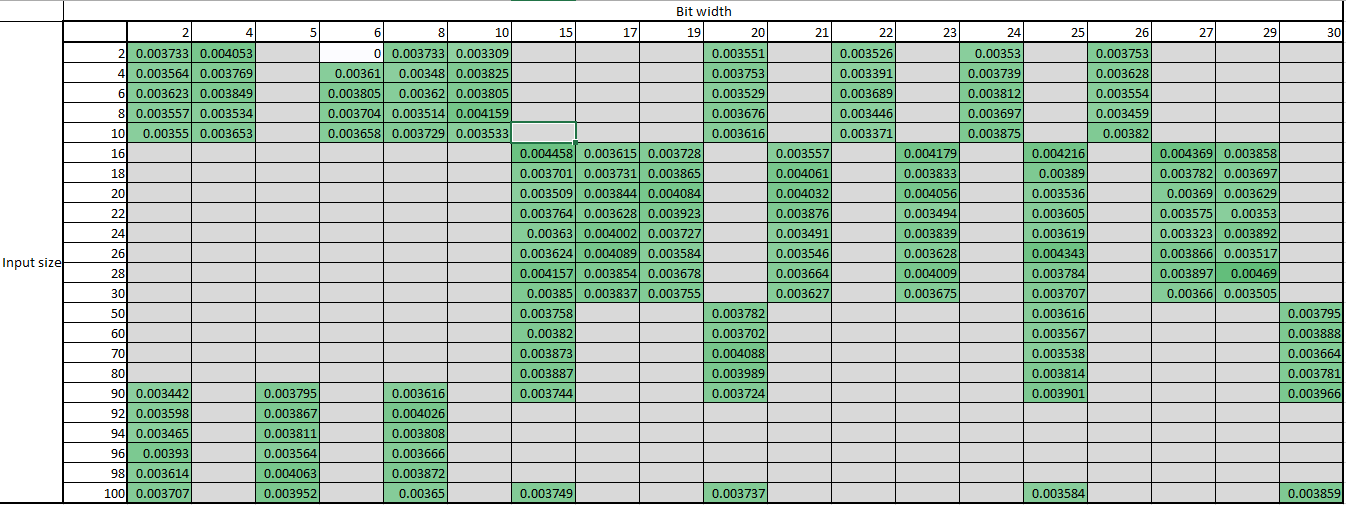
\includegraphics[width=12cm]{p4_LP_rt.png}
\caption{Runtimes for LP subset sum models}
\label{fig:lp_rt}
\end{figure}

\begin{figure}[h]
\centering
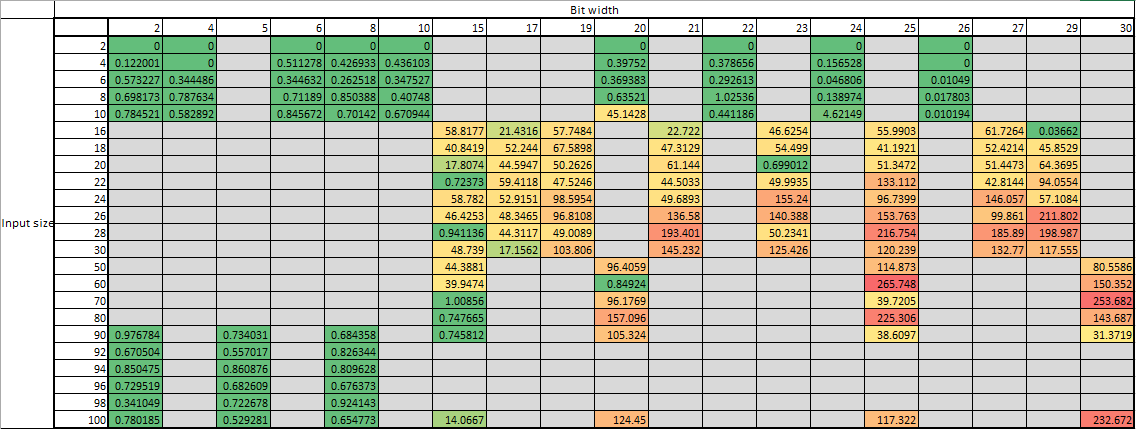
\includegraphics[width=12cm]{p4_ILP_rt.png}
\caption{Runtimes for ILP subset sum models}
\label{fig:ilp_rt}
\end{figure}

\section{Results}

The results are presented in Figure~\ref{fig:ilp} below. The vertical axis represents the
input size and the horizontal axis the word length of the elements in bits.

\begin{figure}[h]
\centering
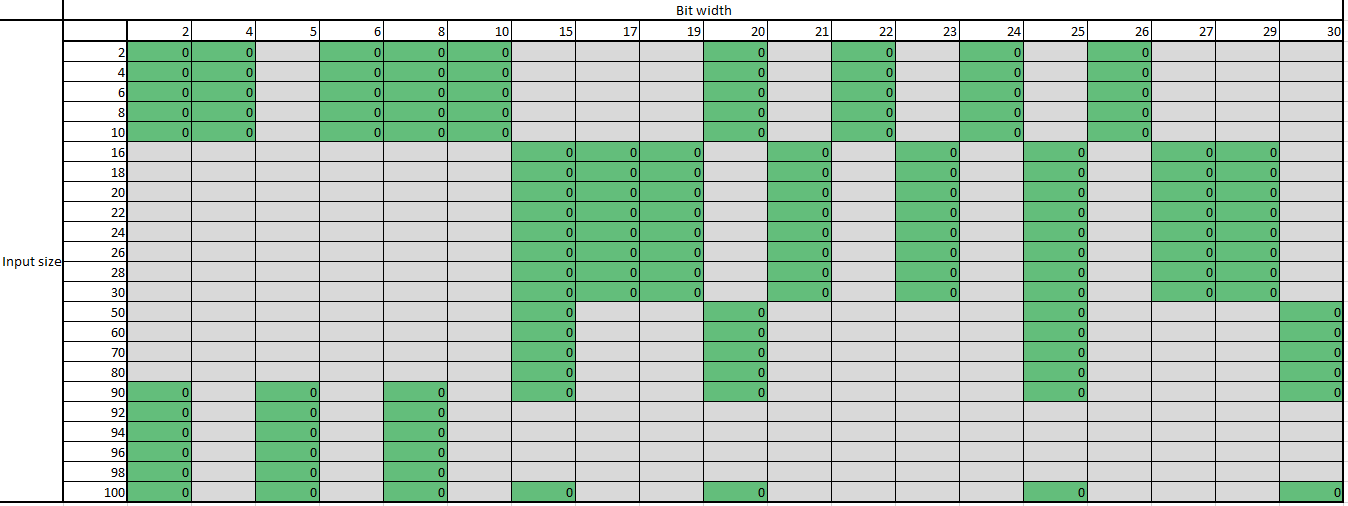
\includegraphics[width=12cm]{p4_ILP_mg.png}
\caption{Margin of error for various input size and word length combinations for ILP}
\label{fig:ilp}
\end{figure}

Each cell in the above figure is color-coded based on the margin of error
the ILP model had in its final solution. This figure is presented mostly to
contrast with the other figures in the section, as it is clear the ILP model
was able to produce an accurate solution in every instance. Comparing this result
with the same figure for the greedy algorithm below, it is abundantly clear
that the ILP approach is vastly superior in terms of accuracy. Note that the
table in Figure~\ref{fig:greedy} uses an accuracy rating that is the inverse of the
ILP table - a rating of 1 is a perfect solution and 0 is instead the worst.

\begin{figure}[h]
\centering
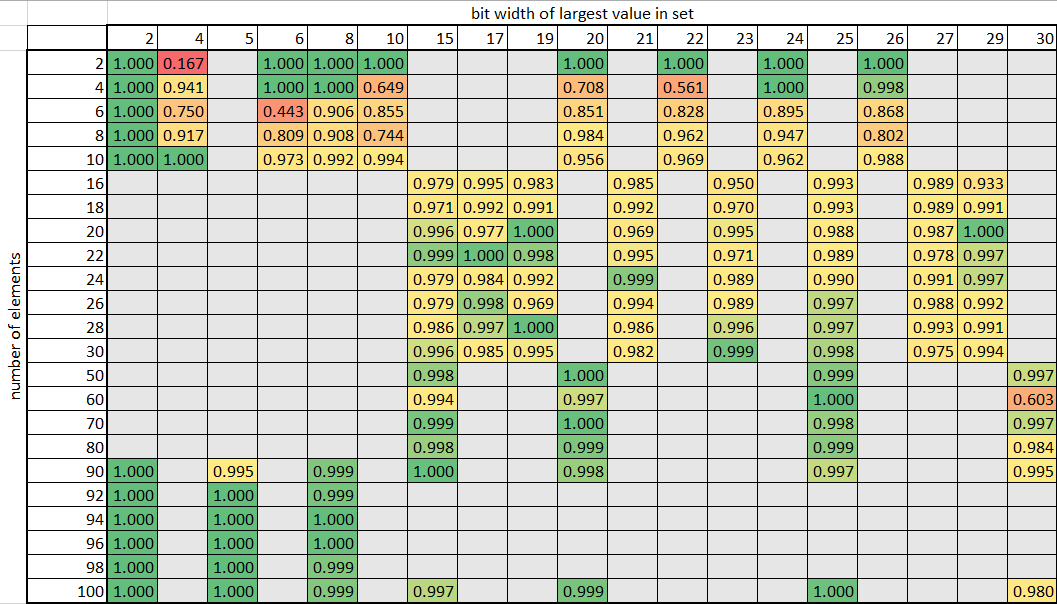
\includegraphics[width=12cm]{P3_margin.png}
\caption{Margin of error for various input size and word length combinations for the greedy algorithm}
\label{fig:greedy}
\end{figure}

Of the 151 instances that were tested, the greedy algorithm was able to
correctly solve 28 of them, yielding an 18.5\% success rate. Compared to the
ILP formulation, which had a 100\% success rate, the greedy algorithm 
is much less successful despite it's lower time complexity. As a reminder,
Figure~\ref{fig:exhaustive} shows the run-times for the exhaustive algorithm.

\begin{figure}[h]
\centering
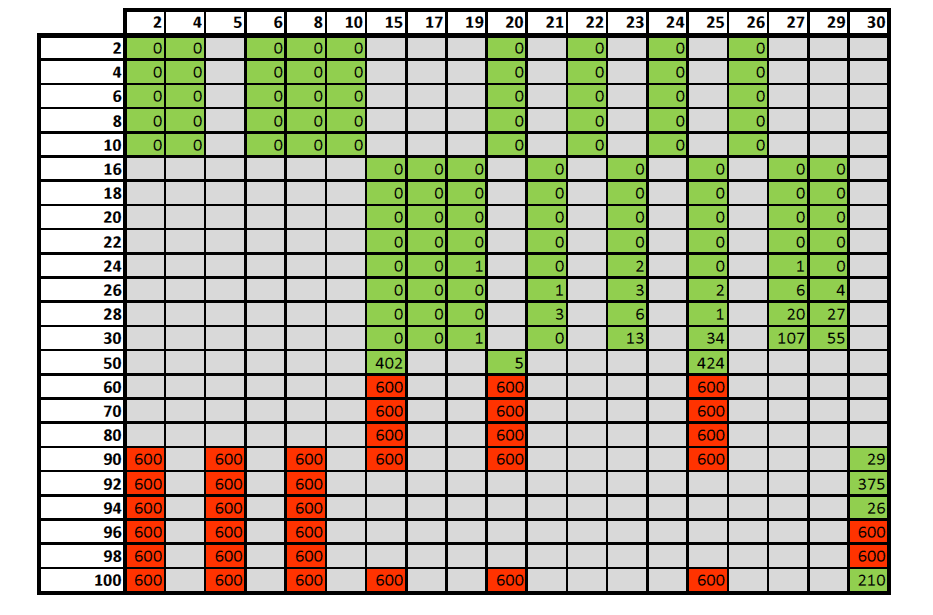
\includegraphics[width=12cm]{P1_res.png}
\caption{Run time for various input size and word length combinations for the exhaustive algorithm}
\label{fig:exhaustive}
\end{figure}

In general, the amount of margin exhibited by the greedy algorithm seems to come down to how many
subsets actually do exist within the set that satisfy the target sum, which depends on factors such 
as the distribution of integers values in the set and whether a value repeats itself.
For example, for sets with several large and small numbers that are similar to each other, there may
be more subsets that satisfy a given target sum compared to a set with a more even distribution of integers.
Granted, this also depends on the target sum itself. But if there are many subsets that satisfy the
target sum, then the greedy algorithm has a better chance of solving a given instance. 

When compared to the exhaustive algorithm, the accuracy advantage of the ILP approach is similar to
that of the greedy algorithm. However, when the timing results of the ILP algorithm in Figure~\ref{fig:ilp_rt}
are compared to that of the exhaustive algorithm, it is actually the much more primitive exhaustive
algorithm that has the advantage in solving smaller or less complex instances. This result was surprising,
as all other findings seemed to indicate that ILP was more or less a 'magic bullet' for solving our
subset sum instances.

\section{Conclusion}

Overall it seems that ILP is a very strong for solving subset sum instances.
More specifically, ILP excels at solving more complex instances that greedy or exhaustive
approaches cannot solve in a reasonable amount of time. However, due to its sophisticated approach to generating
a solution, it seems to be excessively costly for solving simpler instances. In these instances, one can reach
an optimal solution much faster by using a simpler approach. This illustrates that not only is there no perfect 
method to solve any optimization problem, but it seems that often there is no perfect method for solving every
instance of a single optimization problem.

%%%%%%%%%%%%%%%%%%%%%%%%%%%%%%%%%%%%%%%%%%%%%%%%%
% PROJECT 5
%%%%%%%%%%%%%%%%%%%%%%%%%%%%%%%%%%%%%%%%%%%%%%%%%

\chapter{Local Search Algorithms}
In this chapter, we review some of the local search algorithm implementations. One benefit of local search
is that we can choose a neighborhood of possible solutions to explore, and continue exploring until we
either find the best solution in the neighborhood, or we run out of time. 

\section{Finding an Initial Solution}
One requirement for local search algorithms is that they need an initial solution to start from, which
can be generated by any mean. For this project, we chose to generate initial
solutions through the (1) greedy and (2) random algorithm implementations.

\section{Searching a Neighborhood}
The local search algorithms require a neighborhood to be defined as well. We decided to define a neighborhood
via 1-OPT. In this implementation, given an initial solution, we will choose to remove one element in the set
and add another element. In the case of following a steepest descent behavior, we repeat this until we
either ran out of time, or until we reached a case where swapping out any element in the current solution
would only increase the delta between the current sum and the target sum (the goal in this case is to always try to
get closer to the target sum). In that case we have found a locally
optimal solution and stop. Thus, starting with the initial solution found via the greedy and random
algorithms, we take 1-OPT and continue to drill down to the nearest locally optimal solution.

As a point of comparison, we also implemented the tabu algorithm. In this case, we maintain a history
of previous solutions considered, avoiding those solutions when looking for new ones. The general
benefit of this approach is, given a sufficiently large window of history, we can escape ``valleys''
where locally optimal solutions exist, and possibly find an even better solution. In this case,
we kept a history of the past 100 solutions that were considered.

\section{Results}
Given the different approaches to the initial solution, it is possible that this impacted
the locally optimal solution for the instance. This can be expressed as a ratio of the sum of
the locally optimal solution divided by the initial sum was found. Figures ~\ref{fig:greedy_final_initial_compare} and
~\ref{fig:random_final_initial_compare} show the amount of benefit the 1-OPT algorithm was able to
provide over the initial solutions that were found. In general, neither algorithm provided a significant advantage over
the other. That said, the instances that show the largest benefit were typically low density (i.e. smaller values
and a small number of elements in the set). This is most likely due to the fact that, given fewer numbers in a set and small
numbers in general, adding and removing values is going to have a disproportionate impact on the current sum. Several instances
show a value of 1.00, which means that the initial solution was actually sufficient. Ignoring the top-left region and the instances
that showed no benefit, the remaining instances generally show only minor improvements.

It appears that the random algorithm did help some of the smaller density instances. Interestingly enough, given
the random algorithm, it actually led to some cases where the instance could not be solved. This would mean
that there there no solution that contained n elements, as selected in the initial solution. In that case the ``landscape''
was flat, with no locally optimal solution in the neighborhood.

On average, starting with the initial solution found via the greedy algorithm, 1-OPT was able to generate a solution
with a sum that was 1.073 times larger on average. When the random algorithm was used instead, 1-OPT was able to come up
with a solution that was 1.126 times larger than the initial solution on average. Note that we will not exceed the target sum.
So, on average, starting with the solution generated via random
was better. This may be do to the fact that with the greedy algorithm, there is little room for diversification.

\begin{figure}[h]
  \centering
  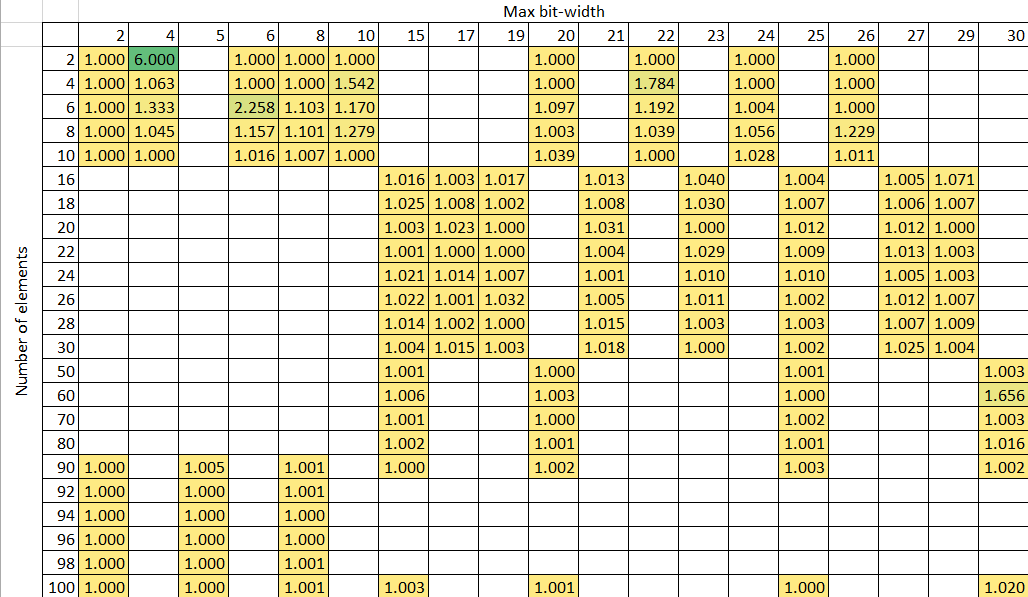
\includegraphics[width=12cm]{p5_greedy_final_over_initial.png}
  \caption{Improvement of final sum over intial sum found via greedy algorithm}
  \label{fig:greedy_final_initial_compare}
\end{figure}

\begin{figure}[h]
  \centering
  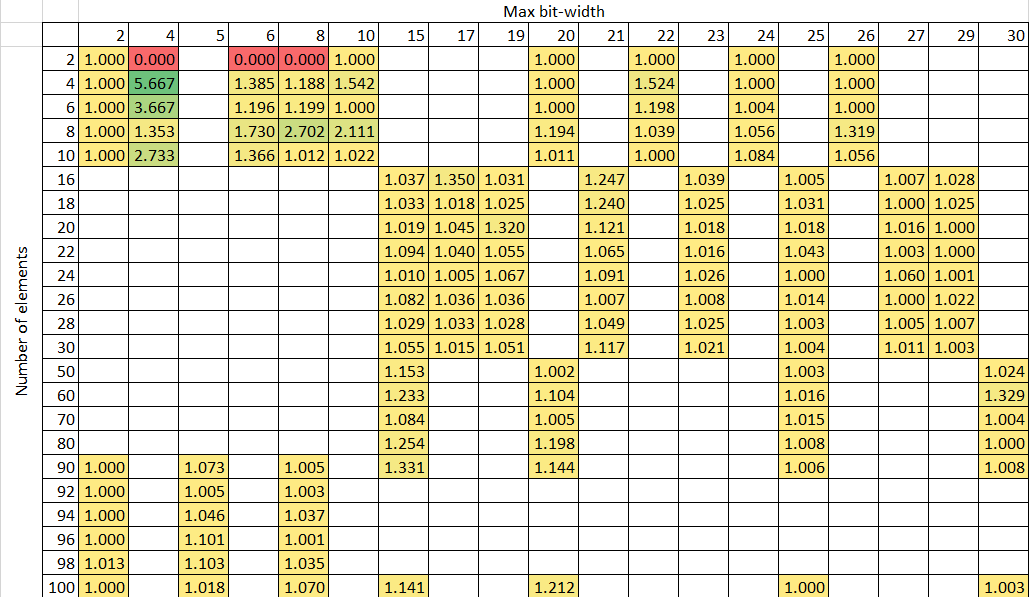
\includegraphics[width=12cm]{p5_random_final_over_initial.png}
  \caption{Improvement of final sum over intial sum found via random algorithm}
  \label{fig:random_final_initial_compare}
\end{figure}

Figure ~\ref{fig:tabu_final_initial_compare} shows the benefit provided by the tabu algorithm.
Note that, compared to the random algorithm, a locally optimal solution was found for each instance. On average,
the final sum found in the tabu algorithm was 1.073 times larger than the initial solution. This is actually similar
to the greedy algorithm, and technically worse on average than the random algorithm. This may be due to not using
a large enough window, leading us to slip back down into the original valley and settle on the locally optimal solution there.
This would imply relatively steep valleys, which is interesting given the improvements shown in the random algorithm
imply large ``flat'' areas where there is no locally optimal solution (or, technically where all solutions are locally optimal).
In terms of the shape of the landscape in general, it would appear that, depending on the density of the instance,
the can be very flat areas where local search fails, and very steep areas where a significantly large window is needed
by tabu in order to find another valley (and thus another possible locally optimal solution).

\begin{figure}[h]
  \centering
  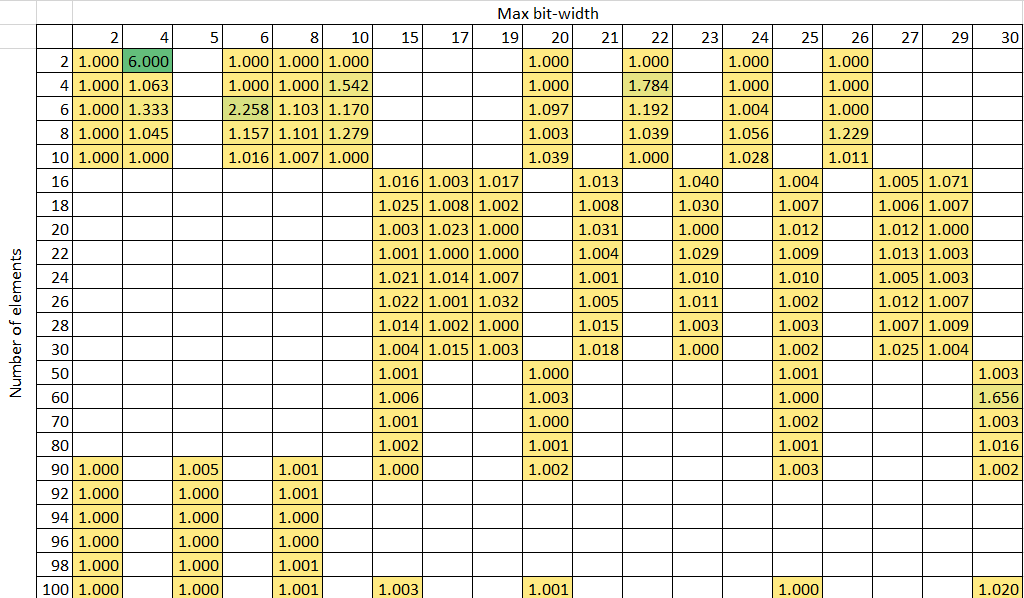
\includegraphics[width=12cm]{p5_tabu_final_over_initial.png}
  \caption{Improvement of final sum over intial sum using Tabu}
  \label{fig:tabu_final_initial_compare}
\end{figure}

The 

\chapter{Conclusion}
Nothing yet dawg.

\bibliography{references}
\bibliographystyle{plain}

\end{document}
